\documentclass[12pt]{article}
\setlength{\oddsidemargin}{0in}
\setlength{\evensidemargin}{0in}
\setlength{\textwidth}{6.5in}
\setlength{\parindent}{0in}
\setlength{\parskip}{\baselineskip}

\usepackage{amsmath,amsfonts,amssymb,graphicx, hyperref, float}

\begin{document}

IBEHS 4A03 \hfill Assignment \#2\\
Baoze Lin, Hady Ibrahim

\hrulefill

% Custom numbering for subparts (e.g., 2.1, 2.2)
\renewcommand{\theenumii}{\arabic{enumi}.\arabic{enumii}}

\begin{enumerate}
\item Question 1
  \begin{enumerate}
    % ANSWER TO 1.1
    \item
    The pole-zero maps for \( Y_1(s) \) and \( Y_2(s) \) help us see system stability. 

    - The left plot shows the pole-zero locations for \( Y_1(s) \), which has poles in the left half-plane, indicating a stable system. It is not oscillatory since there are no imaginary parts to the poles. The poles are: $s=0, -2, -3$. \\
    - The right plot for \( Y_2(s) \) shows at minimum 1 pole in the right half-plane, meaning the system is unstable and will have an exponentially growing response. It is oscillatory since there are imaginary parts to the poles. The poles are: $s=0, 2, 1+2i, 1-2i$.

    \begin{figure}[H]
      \centering
      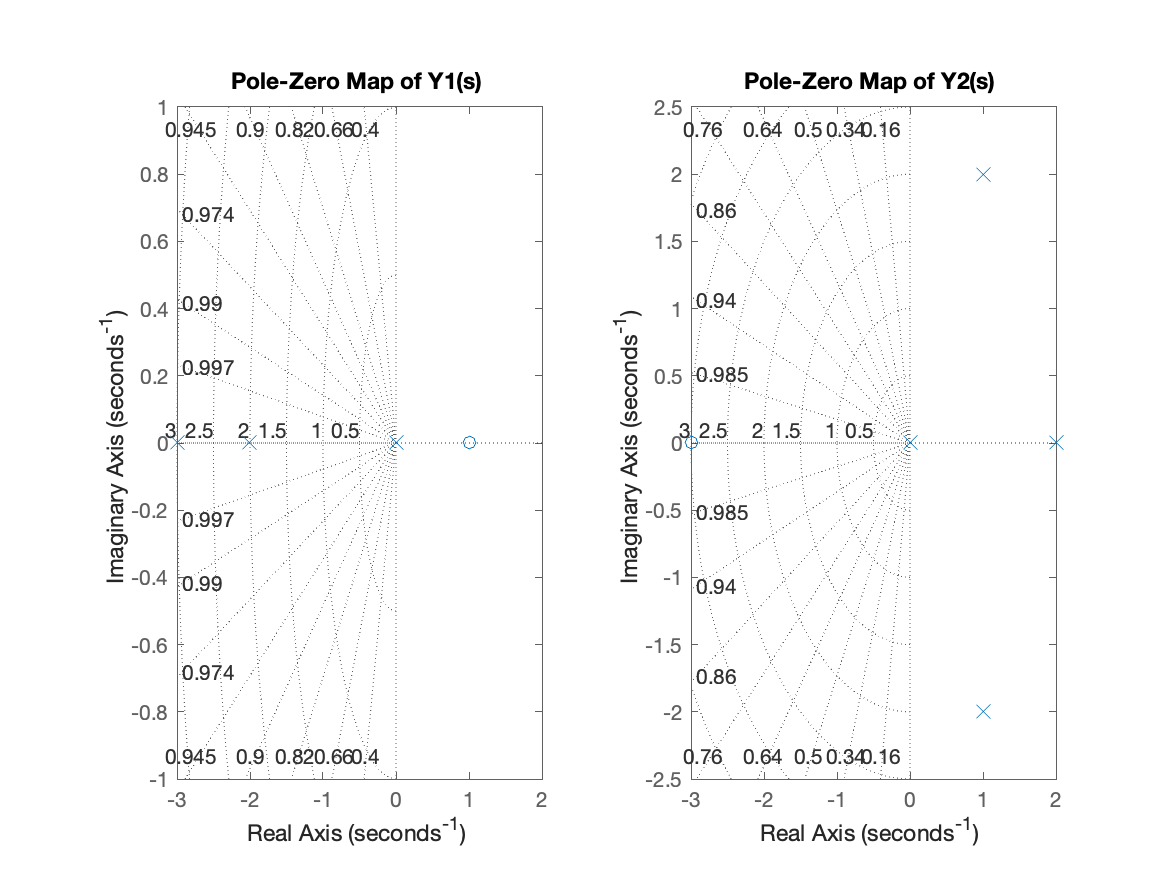
\includegraphics[width=0.8\textwidth]{Figures/figure1-1.png}
      \caption{Pole-Zero Maps for \( Y_1(s) \) and \( Y_2(s) \)}
      \label{fig:figure11} 
    \end{figure}

    \pagebreak
    % ANSWER TO 1.2
    \item
    The Final Value Theorem was used to determine the steady-state values (via hand calculation and using limit() in Matlab):

    \[
    \lim_{t \to \infty} y_1(t) = \lim_{s \to 0} s Y_1(s) = -\frac{1}{6}
    \]

    \[
    \lim_{t \to \infty} y_2(t) = \lim_{s \to 0} s Y_2(s) = -\frac{3}{10}
    \]

    \begin{figure}[H]
      \centering
      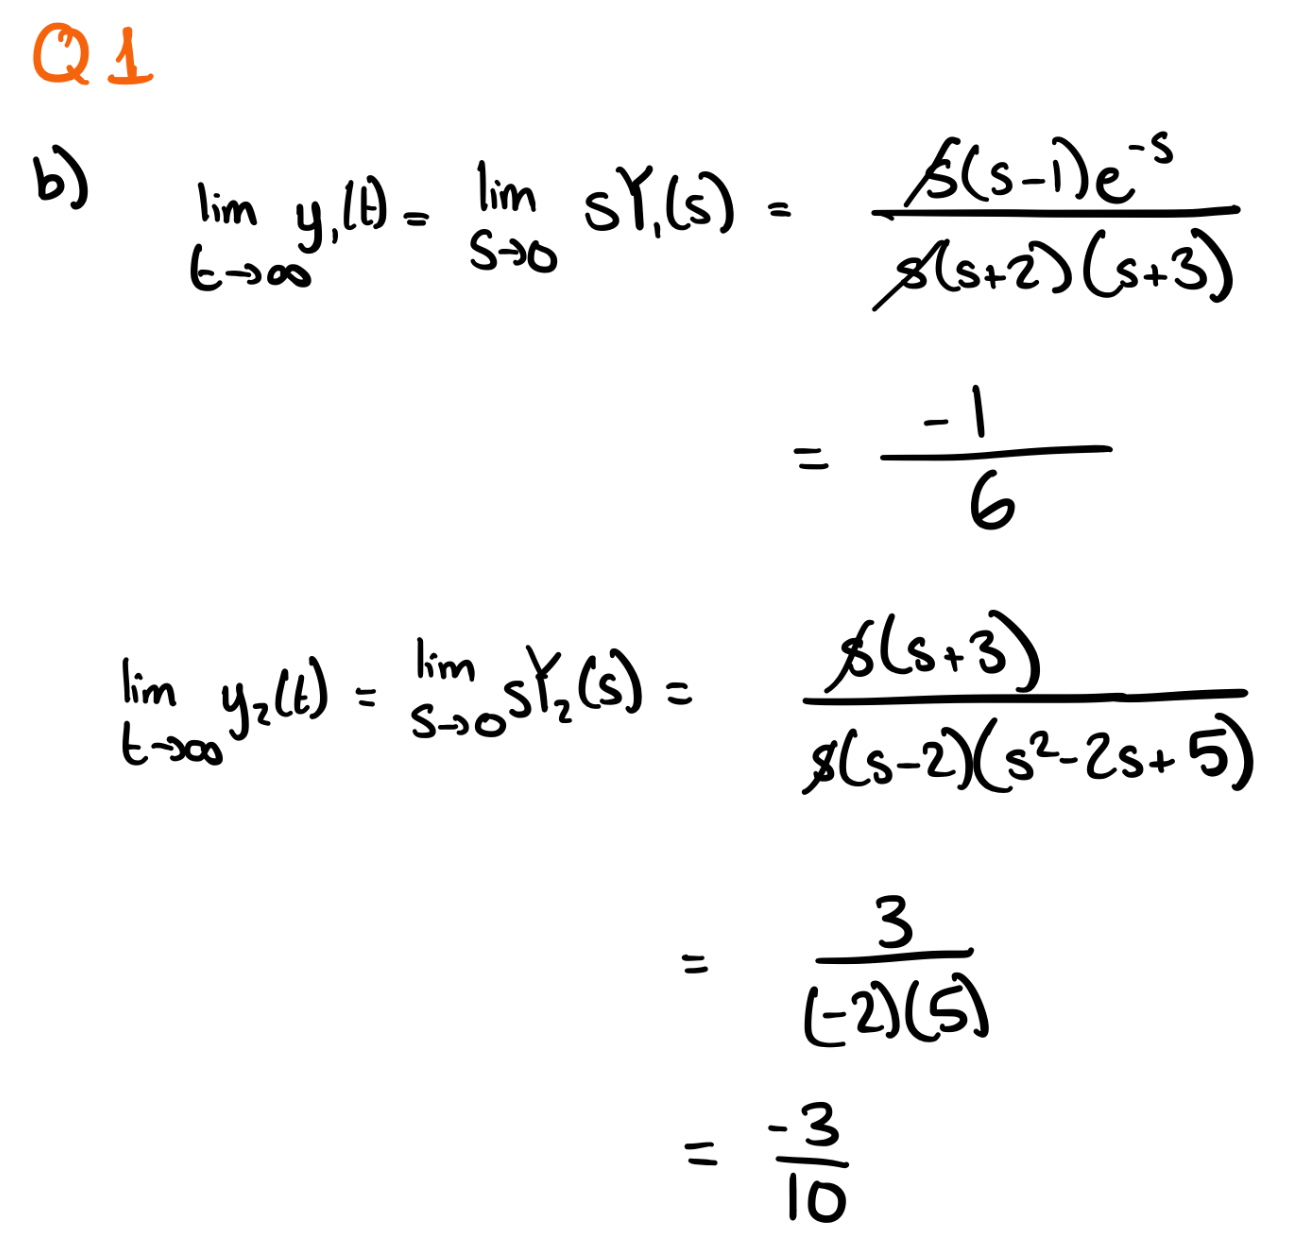
\includegraphics[width=0.6\textwidth]{Figures/handcalc/q1b.png}
      \caption{Final Value Theorem for \( Y_1(s) \) and \( Y_2(s) \)}
      \label{fig:figure14} 
    \end{figure}

    The calculations confirm that \( Y_1(s) \) settles to a finite negative value, whereas \( Y_2(s) \), despite being unstable in impulse response, has a well-defined steady-state when analyzed using Final Value Theorem.

    % ANSWER TO 1.3
    \item
    The impulse response for both systems was computed to observe the effect of the pole locations.

    - The response of \( Y_1(s) \) looks to be bounded confirming stability. \\
    - The response of \( Y_2(s) \) grows exponentially, which aligns with its unstable pole.

    \begin{figure}[H]
      \centering
      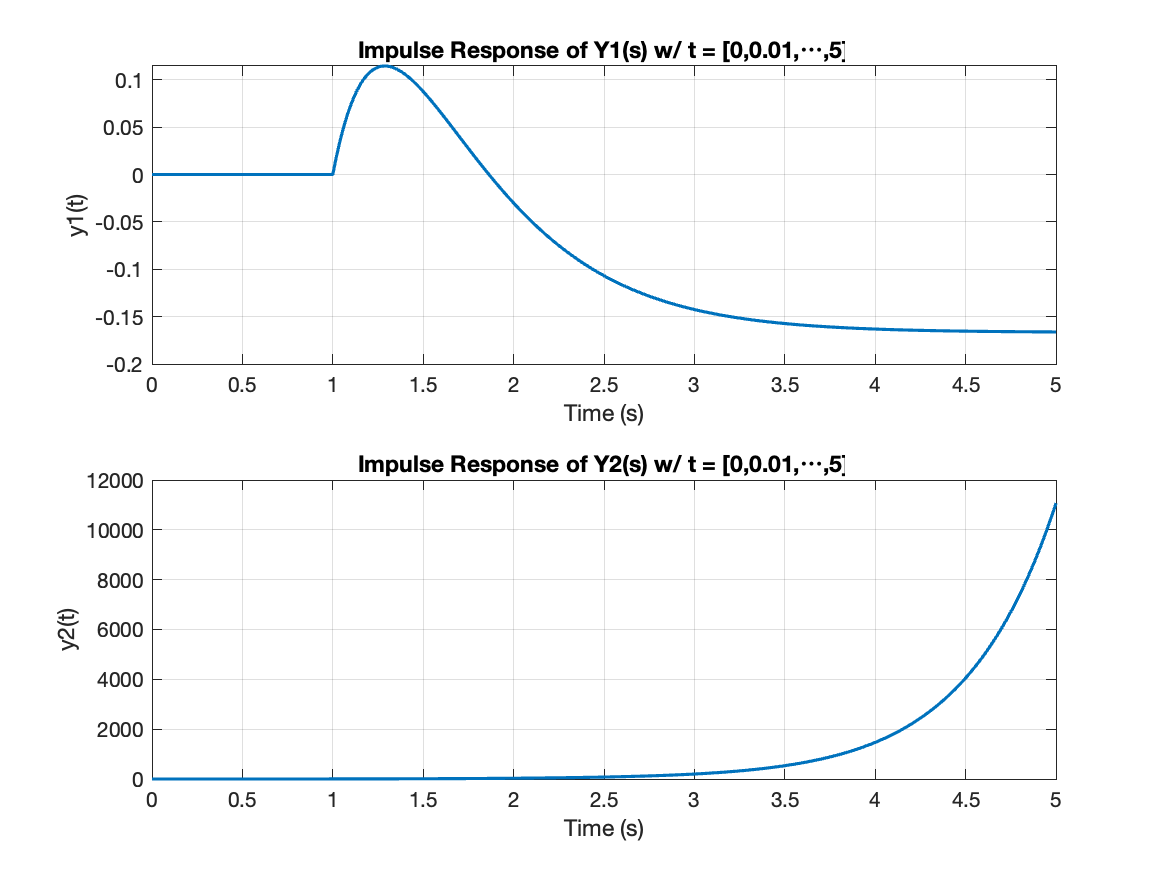
\includegraphics[width=0.9\textwidth]{Figures/figure1-3a.png}
      \caption{Impulse Response of \( Y_1(s) \) and \( Y_2(s) \) for \( t \in [0,5] \)}
      \label{fig:figure12} 
    \end{figure}

    Extending the time range further highlights the unstable growth of \( Y_2(s) \). Not only that, if you zoom into \( Y_1(s) \), you can see that the curve looks a little patchy since the time steps aren't small enough:

    \begin{figure}[H]
      \centering
      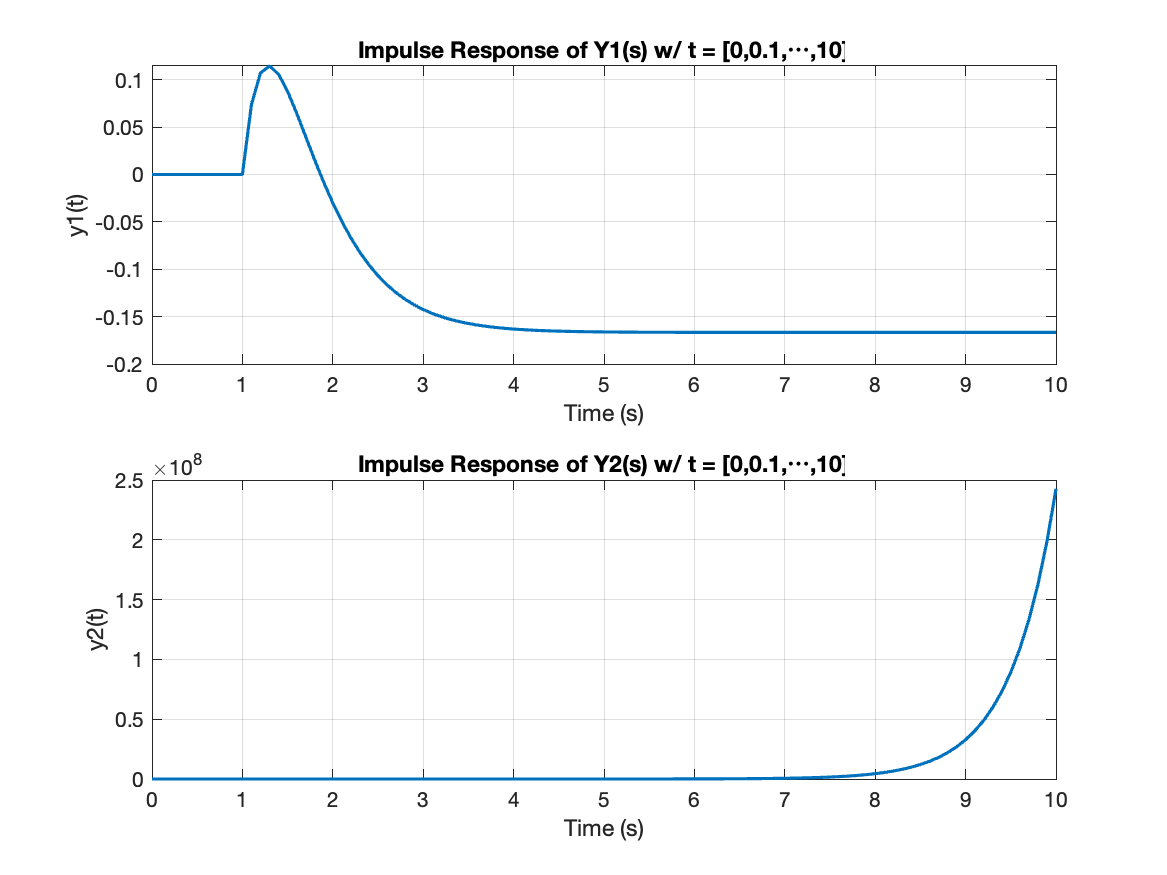
\includegraphics[width=0.9\textwidth]{Figures/figure1-3b.png}
      \caption{Impulse Response of \( Y_1(s) \) and \( Y_2(s) \) for \( t \in [0,10] \)}
      \label{fig:figure13} 
    \end{figure}

  \end{enumerate}

\pagebreak

\item Question 2
  \begin{enumerate}
    % ANSWER TO 2.1
    \item
    Below we've derived the transfer function model that relates the change in temperature of the thermocoupled $T$ to a change in the furnace temperature $T_F$.

    \begin{figure}[H]
      \centering
      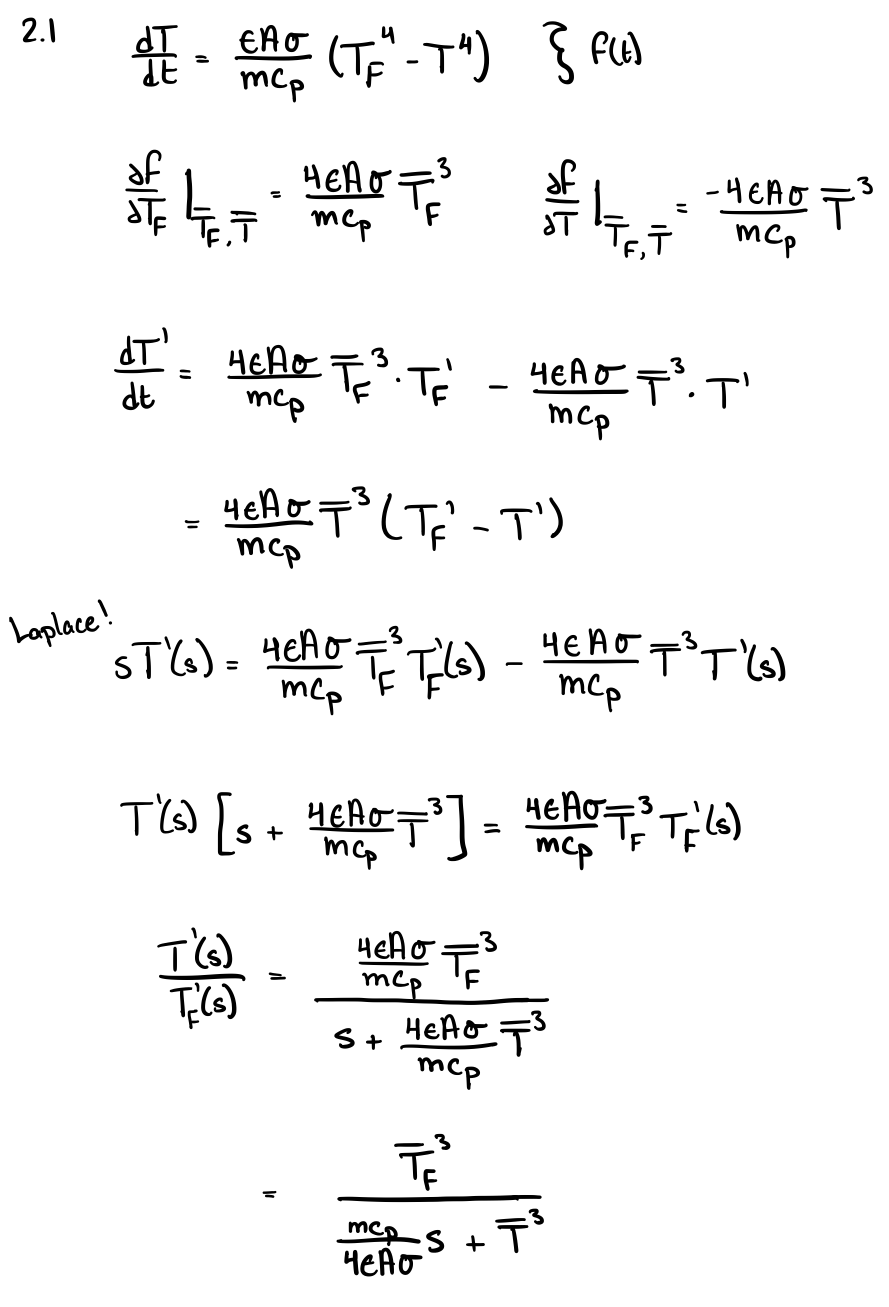
\includegraphics[width=0.6\textwidth]{Figures/handcalc/q2-1.png}
      \caption{Hand calculation to find $T'(s)/T_F'(s)$}
      \label{fig:figure21} 
    \end{figure}

  
    % ANSWER TO 2.2
    \item
    The thermocouple's response to a 30°C drop in furnace temperature was simulated using the linearized transfer function. 
    The step response of the thermocouple shows a gradual decrease in temperature, confirming that the thermocouple lags behind furnace temperature changes.
    The temperature after 10 seconds was 1360.57 K.

    \begin{figure}[H]
      \centering
      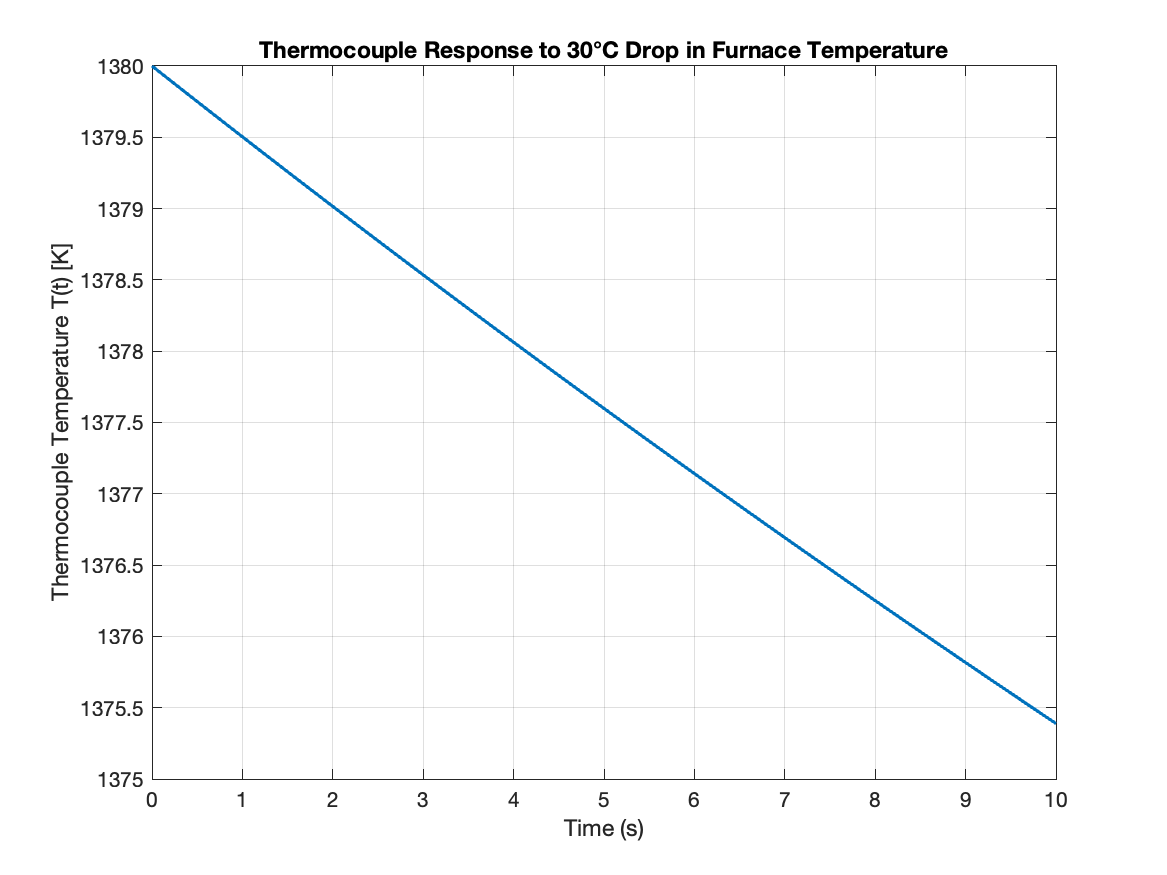
\includegraphics[width=1\textwidth]{Figures/figure2-2.png}
      \caption{Thermocouple Response to 30°C Drop in Furnace Temperature}
      \label{fig:figure22} 
    \end{figure}

    % ANSWER TO 2.3
    \item
    The nonlinear ODE model for the thermocouple temperature was simulated using ode45(). The resulting response follows a slightly curved trajectory, showing a more gradual cooling effect compared to the linearized model. You can see here, that it is very similar to the linearized model, it is a little more rapid towards the start and then slows down as time goes on.
    The temperature after 10 seconds was 1361.07 K.

    \begin{figure}[H]
      \centering
      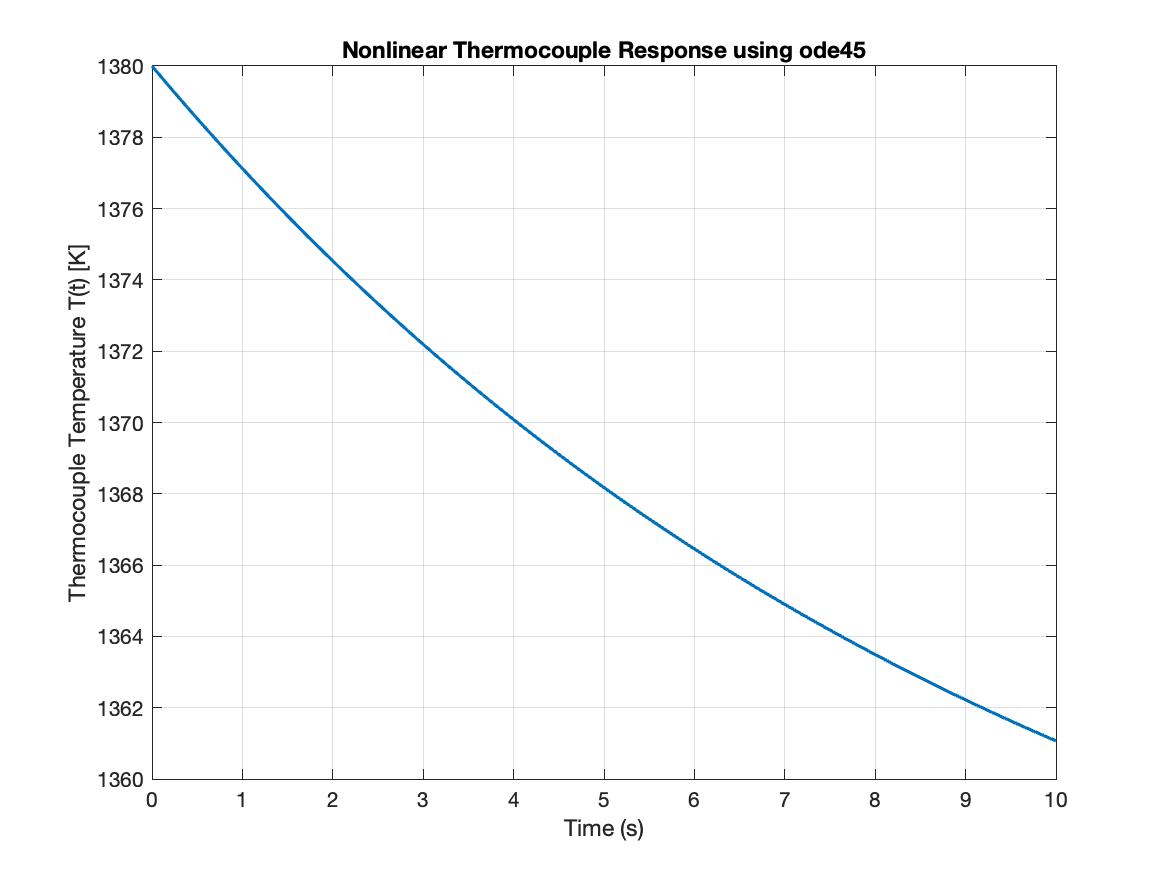
\includegraphics[width=1\textwidth]{Figures/figure2-3.png}
      \caption{Nonlinear Thermocouple Response using ode45}
      \label{fig:figure23} 
    \end{figure}

    % ANSWER TO 2.4
    \item
    Radiative heat transfer follows the Stefan-Boltzmann Law, which is temperature-dependent and nonlinear. This means the rate of heat loss changes more significantly at higher temperatures compared to a simple linear approximation. Due to this, we expected to see that a comparison of the linear and nonlinear models would show that the linearized transfer function underestimates the cooling rate. What we actually saw was that with a -30°C change in temperature, the linearized model predicts a faster response by just a little compared to the non-linear model. With the +30°C change, the non-linear model was a little faster, but again very similar responses. This shows that the linearized model estimated the true temperature quite well. 

    \begin{figure}[H]
      \centering
      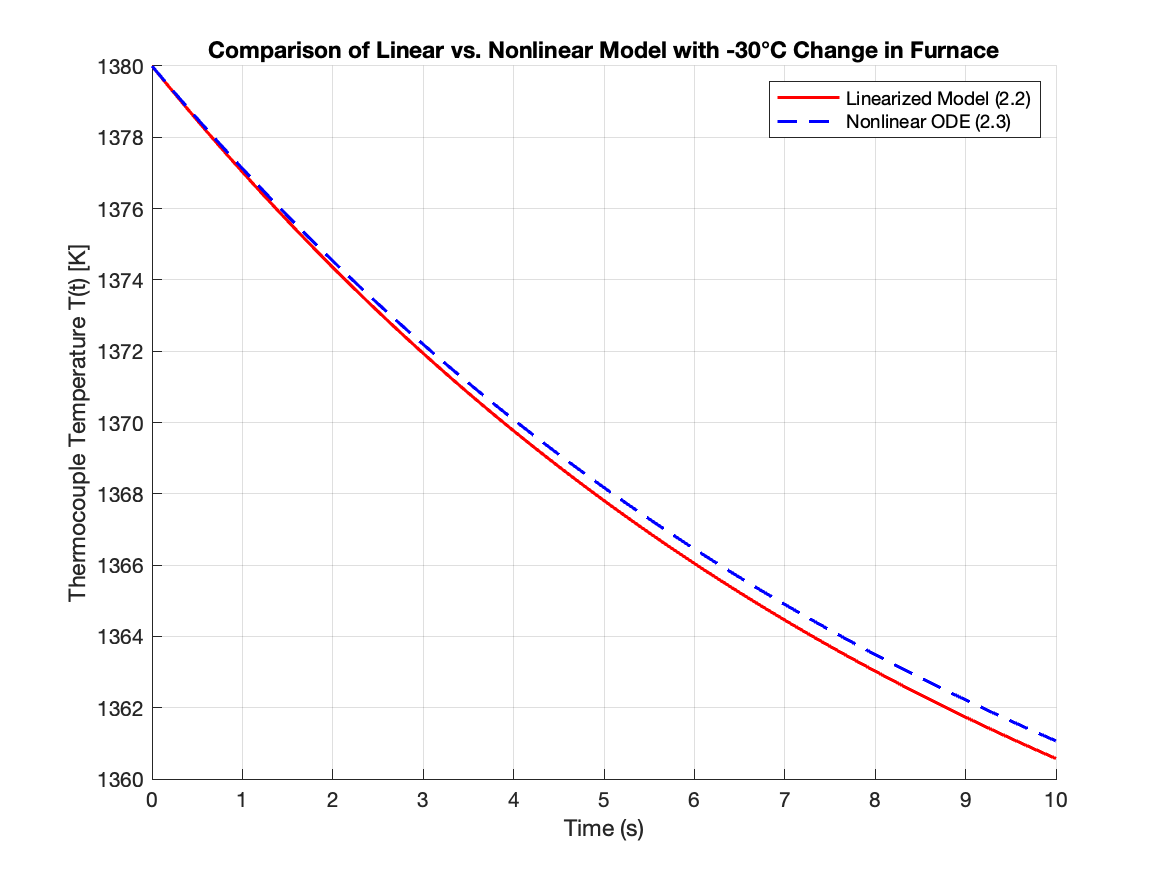
\includegraphics[width=1\textwidth]{Figures/figure2-4a.png}
      \caption{Comparison of Linear vs. Nonlinear Model with +30°C Change in Furnace}
      \label{fig:figure24a} 
    \end{figure}

    \begin{figure}[H]
      \centering
      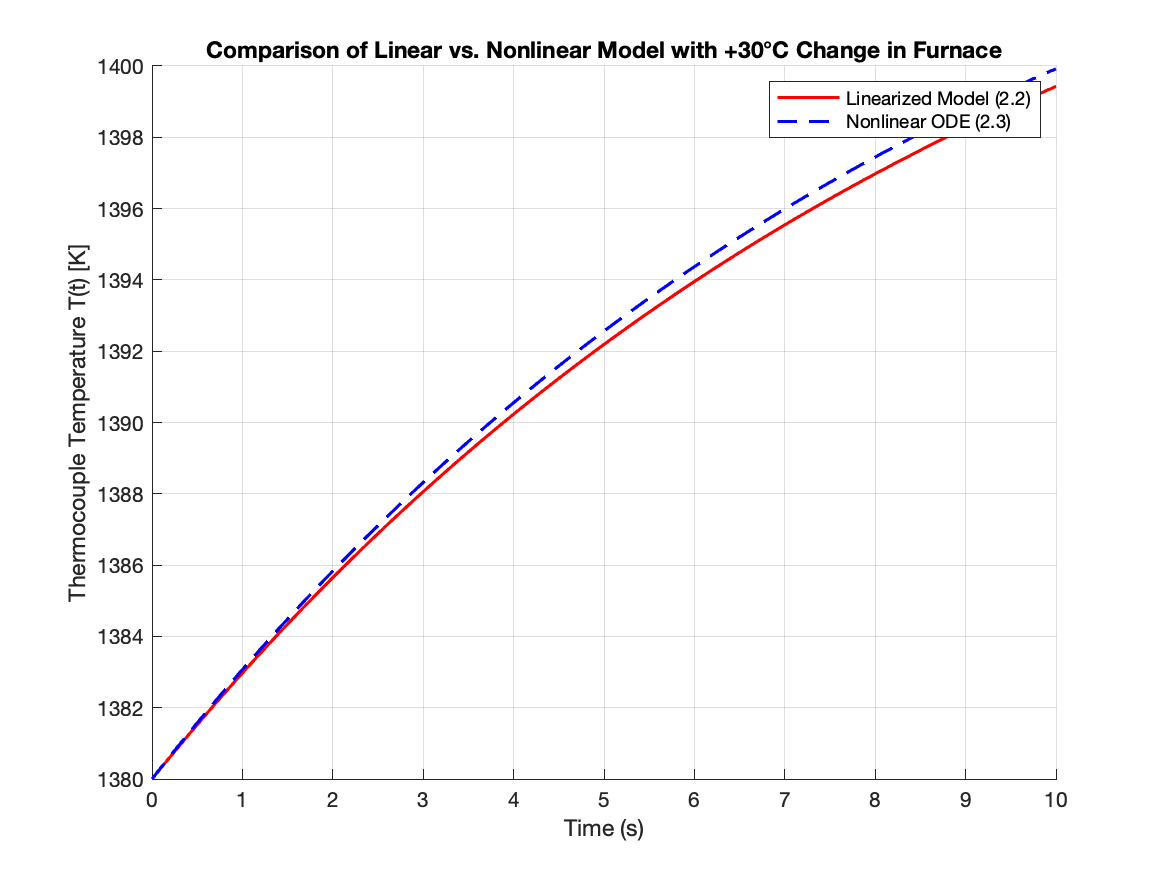
\includegraphics[width=1\textwidth]{Figures/figure2-4b.png}
      \caption{Comparison of Linear vs. Nonlinear Model with -30°C Change in Furnace}
      \label{fig:figure24b} 
    \end{figure}

    % ANSWER TO 2.5
    \item
    In this case, we analyzed the effect of heat input \( Q(t) \) on the thermocouple temperature. The furnace response to \( Q(t) \) was modeled, and the thermocouple's response was calculated by multiplying the transfer functions:

    \[
    \frac{T(s)}{Q(s)} = \frac{T(s)}{T_F(s)} \times \frac{T_F(s)}{Q(s)}
    \]

    The results show that the furnace temperature \( T_F(t) \) increases rapidly in response to the applied heat input and reaches its steady-state value within a few seconds. In contrast, the thermocouple temperature \( T(t) \) rises much more gradually indicating a significant time delay in its response. 

    This delay occurs because the thermocouple absorbs heat primarily through radiation, which is a slower process compared to the direct heating of the furnace. As a result, the thermocouple reading does not immediately reflect the actual furnace temperature, but instead lags behind, converging toward the final temperature over time (which it doesn't even reach in the 10 seconds).

    In control applications, this measurement lag is critical to know because relying solely on \( T(t) \) for feedback could lead to delayed or incorrect adjustments. To improve performance, a control system should account for this delay and maybe add some other elements or logic to work around it.

    \begin{figure}[H]
      \centering
      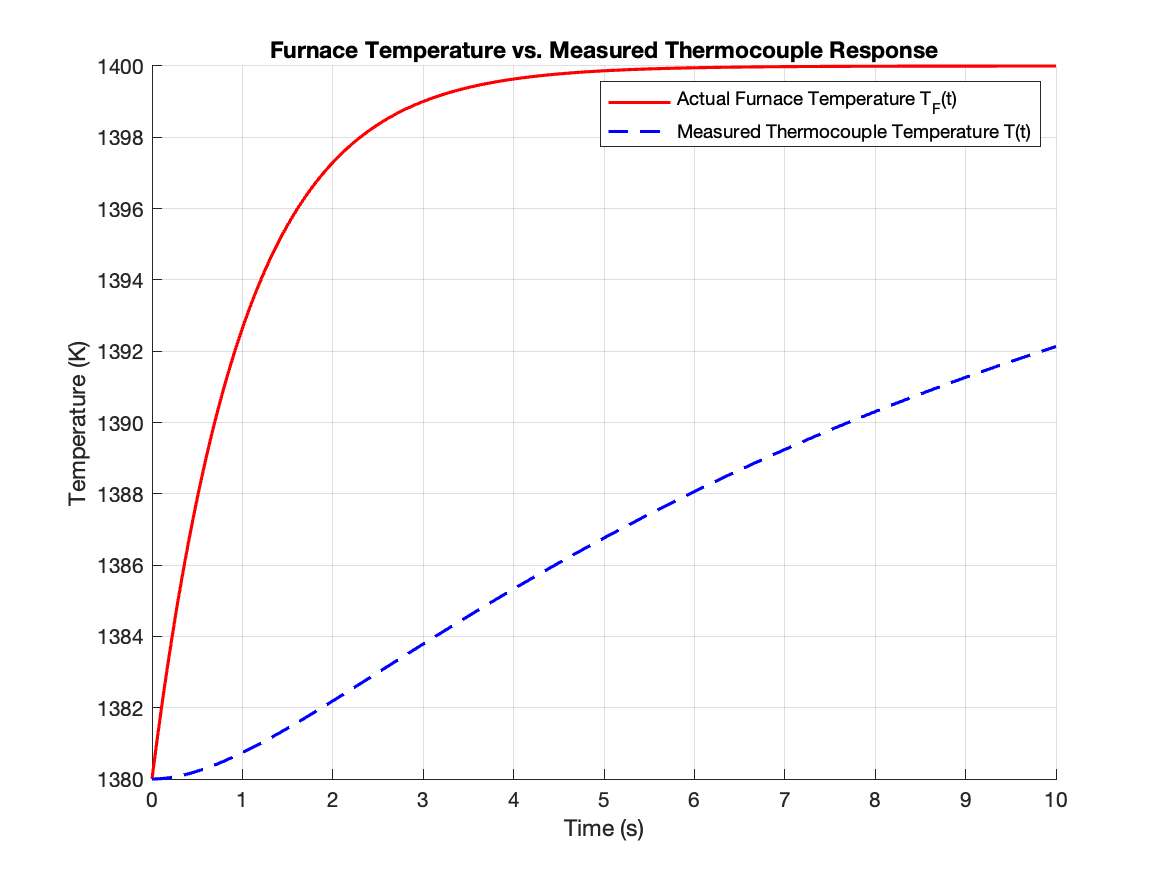
\includegraphics[width=0.7\textwidth]{Figures/figure2-5.png}
      \caption{Furnace Temperature vs. Measured Thermocouple Response with Heat Input \( Q \)}
      \label{fig:figure25} 
    \end{figure}    

  \end{enumerate}

\item Question 3
  \begin{enumerate}
    % ANSWER TO 3.1
    \item 
    The given transfer function is:

    \[
    \frac{V(s)}{P(s)} = \frac{A K_{P \to V}}{\rho A L s^2 + b s + c}
    \]

    To rewrite it in standard form, divide the numerator and denominator by \(c\):

    \[
    \frac{V(s)}{P(s)} = \frac{\frac{A K_{P \to V}}{c}}{\frac{\rho A L}{c}s^2 + \frac{b}{c}s + 1}
    \]

    Let:

    \[
    K = \frac{A K_{P \to V}}{c}, \quad \tau^2 = \frac{\rho A L}{c}, \quad 2\zeta\tau = \frac{b}{c}
    \]

    The transfer function in standard form becomes:

    \[
    \frac{V(s)}{P(s)} = \frac{K}{\tau^2 s^2 + 2\zeta\tau s + 1}
    \]

    % ANSWER TO 3.2
    \item
    The process gain \(K\) relates the steady-state change in the output voltage (\(V(t)\)) to the steady-state change in the input pressure (\(P(t)\)). From both the step test diagram given in the assignment and also Empirical\_Data.csv, we observe the a steady-state output voltage of around 20 mV when the input pressure step test is 2 units. Since the process gain \(K\) is defined as:

    \[
    K = \frac{\Delta V}{\Delta P}
    \]

    Substituting the given values:

    \[
    K = \frac{20}{2} = 10
    \]

    Thus, the process gain for this system is \(K = 10\).

  \end{enumerate}

\end{enumerate}

\end{document}
